\documentclass[a4paper,10pt]{report}
\usepackage[T1]{fontenc}
\usepackage{framed}
\usepackage{graphicx}
\usepackage[utf8]{inputenc}
\usepackage[italian, english]{babel}
\usepackage{geometry,setspace,listings,graphicx,lettrine,float,hyperref,eurosym,fancyhdr,booktabs,bookmark,titling}
\usepackage[dvipsnames]{xcolor}

\graphicspath{ {../images/} }

\renewcommand*\footnoterule{}
\geometry{a4paper,top=3cm,bottom=3cm,left=3cm,right=2.5cm}
\singlespacing

\fancypagestyle{plain}
{
	\fancyhf{}
	\rfoot{\thepage}
}
\pagestyle{fancy}
{
	\fancyhf{}
	\headsep=40pt
	\lhead{\slshape \rightmark}
	\rhead{\slshape \leftmark}
	\rfoot{\thepage}
}
\begin{document}
  \thispagestyle{empty}
  \enlargethispage{60mm}
  \begin{center}
    \Large{\textsc{Università degli studi di Napoli Parthenope}}\\
    \large{Corso di laurea in Informatica}\\
    \large{Dipartimento di Scienze e Tecnologie}\\
    \vspace{25mm}
    \textbf{\Huge{\textsc{Bitcoin}}}\\
    \Large{Progetto d'esame Reti dei Calcolatori}\\
    \vspace{7mm}
    \begin{figure}[h]
    	\begin{center}
    	   
\includegraphics[scale=0.2]{parthenope.jpeg}
      \end{center}
    \end{figure}
    \vspace{35mm}
    \textbf{Vittorio FONES 0124/1384}
    
    \textbf{Vittorio ZAVINO 0124/1241}\\
    \vspace{5mm}

    \large{A. A. 20018-2019}
  \end{center}

  \pagenumbering{Roman}


  \tableofcontents
  \listoftables
  \listoffigures
  \lstlistoflistings

  \chapter{Descrizione del progetto}
  \pagenumbering{arabic}
  
  \lettrine[lraise=0.1]{C }on il seguente elaborato illustriamo il lavoro svolto per la realizzazione del progetto Bitcoin, il cui scopo è quello di creare una rete peer to peer usata per la gestione di una blockchain e l'utilizzo della stessa. Il progetto è stato sviluppato nel linguaggio C, attenendoci allo standard Posix come illustrato durante il corso e sul libro GAPIL: per l'appunto il software gira anche sotto piattaforma Mac OS, oltre che su distrubuzioni Linux quali Debian e Arch Linux.\newline Di seguito viene allegata l'introduzione della traccia sviluppata:
  \begin{framed} Si vuole realizzare un sistema per la gestione di una criptovaluta basato su una rete P2P. Il sistema è basato sulla gestione di una blockchain, ovvero una sequenza di blocchi in cui ogni blocco contiene una transazione. Il sistema si compone di due tipi di nodi: NodiN e NodiW. I NodiN creano la rete P2P e gestiscono la blockchain. Inoltre stampano la blockchain ogni volta che viene aggiunto un blocco: (blocco 1 )- > (blocco 2 )- > (blocco 3 )- > (blocco 4 ). I NodiW gestiscono i wallet (portafogli virtuali) che consentono di inviare e ricevere pagamenti. Ad ogni nuovo pagamento inviato o ricevuto il nodo stampa la transazione ed il totale del portafogli. 
\end{framed}
Da adesso in avanti, i nodiN e nodiW saranno definiti rispettivamente \textbf{peer} e \textbf{wallet}.
\\ Seguendo poi la descrizione dettagliata abbiamo considerato l'accoppiata [IP:porta], definita da adesso in poi come net_ent, che i wallet utilizzano per connettersi ai peer, come loro identificativo nelle transazioni.\\
Mentre come ID di una transazione si è usata una stringa univoca fornita da una apposita funzione, consistente nella concatenazione del time_stamp, net_ent mittente(src), net_ent(dst) e ammount della transazione. 

  \chapter{Descrizione e schemi dell'architettura}
  Attraverso l'utilizzo di un server centrale si è deciso di implementare una rete P2P Hybrid Decentralized.
\\Quindi i nodiN e i nod
\\Un peer, ovvero un nodoN, per entrare nella rete chiederà al server principale di fornigli ip e porta di altri peer e tenterà l'aggancio a loro. In modo simile il wallet, ovvero il nodoW, si collegherà alla rete dopo che il server principale gli fornirà l'ip e porta del peer a cui connettersi. Ovviamente tale funzionalità di aggancio viene sfruttata qualora un peer o un wallet dovessero crashare.
È stato scelto di non mantenere informazioni specifiche della rete quali la struttura del grafo per cercare di portare avanti l'ideale di decentralizzazione dell'informazione. Questa archittetura non è esente da problemi, infatti un eventuale crash improvviso del server porta ad uno stato di disordine della rete ed ad un decadimento della stessa. Per tale motivo la chiusura del server principale da parte del 'sistemista' fa chiudere in maniera pulita tutti i peer e wallet associati.
  \begin{figure}[H]
  \center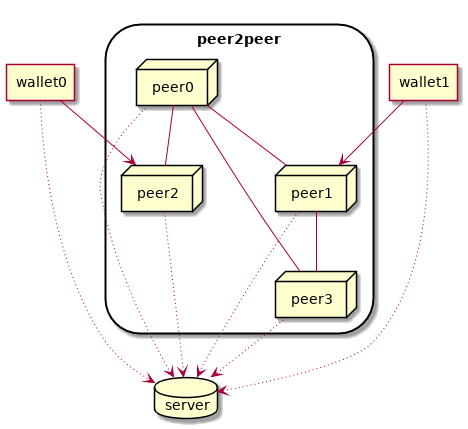
\includegraphics[scale=0.50]{arch.png}
  \caption{Architettura di sistema.}
  \end{figure}
  

 
  \chapter{Descrizione e schemi del protocollo applicazione}
  Di seguito sono riportati gli schemi dei principali protocolli applicazione.
  \section{Primo aggancio e creazione della rete}
  Per creare la rete Peer to Peer sarà necessario lanciare il server che è in perenne attesa di codici hash crittografati con hash256. Autentificati, i client, verrano risposti con un numero di peer a cui collegarsi e da i rispettivi indirizzi ip e porte. Il server a seguito di una risposta positiva salverà il peer nella propria lista, in modo da poter aumentare l'espasione del grafo.
 Un nodo peer correttamente agganciato ad un suo simile, avvierà una procedura di sincronizzazione della blochchain.
  \begin{figure}[H]
  \center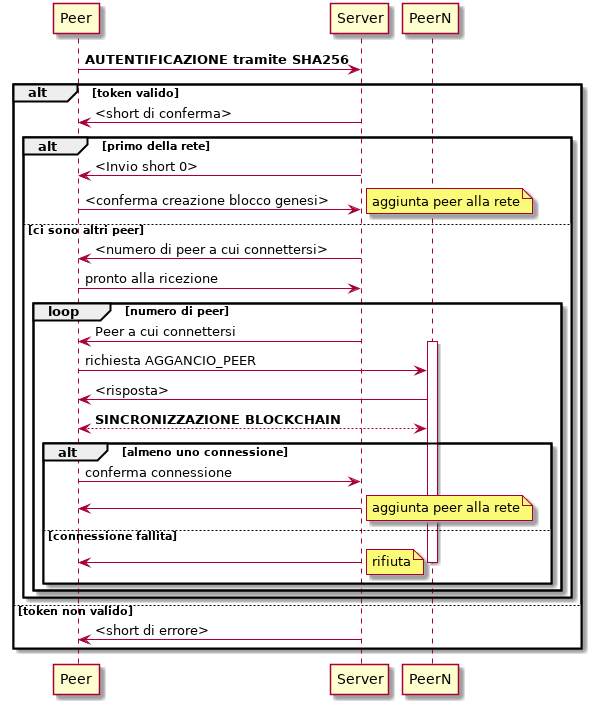
\includegraphics[scale=0.40]{hookpeer.png}
  \caption{Aggancio peer.}
  \end{figure}
  
  \section{Aggancio wallet.}
  La procedura dell'aggancio del wallet è in parte simile a quella del peer. Dopo l'autentificazione con il server e ricevuto il peer, il wallet si connetterà a quest'ultimo, mentre il peer lo inserirà nella propria lista.
  \begin{figure}[H]
  \center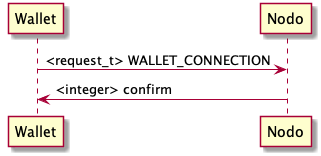
\includegraphics[scale=0.40]{hookwallet.png}
  \caption{Aggancio wallet.}
  \end{figure}
  
  
  \chapter{Dettagli implementativi}
    

    \section{Dettagli del server}\noindent
Il server è stato scelto di implementarlo come un normale server iterativo: ogni richiesta verrà evasa al termine della precedente garantendo la creazione della rete in maniera omogenea.


 
n Per la realizazione di ogni applicativo si è optato per protocolli TCP/IP e Socket di Berkley. Particolare importanza è stata data alla struttura del progetto che è reso modulare tramite le opportune librerie, indipendenti ed usabili per altri scopi.

    \section{Dettagli del peer}\noindent
 I peer poiché devono spedire i vari blocchi, controllare la validità degli stessi, servire le richieste di bilancio e di transazione dei wallet, sono stati implementati secondo uno schema I/O Multiplexing che usa i thread posix della libreria pthread. Essendo il cuore portate della rete un peer è composto da due parti: un server che permette ai vari thread di connettersi attraverso la propria porta di servizio, scelta da riga di comando, ed un client.
Per ovviare ai relativi problemi dovuti all'accesso concorrente alla lista si è scelto di sincronizzare i thread tramite mutex, e semafori binari: tale schema ricorda il paradigma dei Lettori/Scrittori.

    \section{Dettagli del wallet}\noindent
    
 I nodi wallet dovendo gestire input da tastiera e l'arrivo dalla rete di richieste dal peer connesso, si è deciso di implementarlo con uno schema I/O Multiplexing.

    

  \chapter{Manuale utente}

  \section{Instruzioni per la compilazione}\noindent



  \section{Instruzioni per l'esecuzione}\noindent

\end{document}
